\documentclass{article}
\usepackage{graphicx}
\usepackage[margin=1in]{geometry}
\usepackage{amsmath,amssymb}
\usepackage{float}
\usepackage{booktabs}

\setlength{\parindent}{0pt}
\setlength{\parskip}{0.5em}

\title{Hohmann Transfer via Sequential Convex Programming}
\author{Hudson Kim}
\date{November 2026}

\begin{document}
\maketitle

\section{Orbital Dynamics}

Suppose a spacecraft starts in a circular orbit and we want to transfer it to a higher circular orbit. We will use two impulsive burns, one to enter the transfer orbit and another to circularize at the final orbit. Between the burns, the spacecraft follows two-body dynamics.

Define the state as
\[
\vec{x}=\begin{bmatrix}x&y&v_x&v_y\end{bmatrix}^{T},
\]
where $x$ and $y$ are position in km and $v_x$ and $v_y$ are velocity in km/s. Let $r=\sqrt{x^2+y^2}$ be the distance from Earth's center and let $\mu=398600.44\ \mathrm{km^3/s^2}$ be Earth's gravitational parameter. Then
\[
\boxed{
\dot{\vec{x}}=f(\vec{x})=
\begin{bmatrix}
 v_x\\
 v_y\\
 -\mu x/r^3\\
 -\mu y/r^3
\end{bmatrix}.}
\]

We use the following orbital radii:
\[
r_1=6569.487\ \mathrm{km},\qquad r_2=42159.137\ \mathrm{km}.
\]
These correspond to an initial altitude of $191.35$ km and a final altitude of $35781$ km.

\section{Boundary Conditions}

We want to solve for the two burns, $\Delta\vec{v}_1$ and $\Delta\vec{v}_2$, where each is a two-dimensional change in velocity (km/s). We discretize the transfer into $N$ states, $\vec{x}_0,\ldots,\vec{x}_{N-1}$.

The first state is defined \emph{after} the first burn. Since an impulsive burn changes velocity but not position, we have
\begin{align*}
\begin{bmatrix}x_0\\y_0\end{bmatrix}
&=\begin{bmatrix}0\\-r_1\end{bmatrix},\\
\begin{bmatrix}v_{x,0}\\v_{y,0}\end{bmatrix}
&=\begin{bmatrix}\sqrt{\mu/r_1}\\0\end{bmatrix}+\Delta\vec{v}_1.
\end{align*}

Likewise, the last state is defined \emph{before} the second burn. Ideally, it should be at $(0,r_2)$, and the second burn should give the spacecraft the circular velocity of the final orbit:
\begin{align*}
\begin{bmatrix}x_{N-1}\\y_{N-1}\end{bmatrix}
&=\begin{bmatrix}0\\r_2\end{bmatrix}+\vec{s}_r,\\
\begin{bmatrix}v_{x,N-1}\\v_{y,N-1}\end{bmatrix}+\Delta\vec{v}_2
&=\begin{bmatrix}-\sqrt{\mu/r_2}\\0\end{bmatrix}+\vec{s}_v.
\end{align*}

Here $\vec{s}_r$ is a terminal position slack (km) and $\vec{s}_v$ is a terminal velocity slack (km/s). We allow these errors during the SCP iterations and penalize them in the objective. For the final solution, both should be close to zero.

\subsection{Analytical Reference}

We can compare the numerical result against the analytical Hohmann transfer. The semimajor axis of the transfer ellipse is
\[
a_t=\frac{r_1+r_2}{2}.
\]
Using the vis-viva equation, the two burn magnitudes are
\begin{align*}
\Delta v_{H,1}
&=\sqrt{\mu\left(\frac{2}{r_1}-\frac{1}{a_t}\right)}
 -\sqrt{\frac{\mu}{r_1}},\\
\Delta v_{H,2}
&=\sqrt{\frac{\mu}{r_2}}
 -\sqrt{\mu\left(\frac{2}{r_2}-\frac{1}{a_t}\right)}.
\end{align*}

The spacecraft travels half of the transfer ellipse, so the transfer time is
\[
t_H=\pi\sqrt{\frac{a_t^3}{\mu}}.
\]
For our orbits, this gives
\[
\boxed{\Delta v_H\approx3.935\ \mathrm{km/s},\qquad t_H\approx5.26\ \mathrm{h}.}
\]

\section{Sequential Convex Programming}

The dynamics are nonlinear because gravitational acceleration depends on the spacecraft's position. To use convex optimization, we approximate them around a reference trajectory.

Let $\bar{\vec{x}}_k$ be the reference state at time step $k$. Using a first-order Taylor expansion,
\[
\boxed{
f_{\mathrm{lin},k}(\vec{x}_k)
=f(\bar{\vec{x}}_k)+A_k(\vec{x}_k-\bar{\vec{x}}_k),
}
\]
where
\[
A_k=\left.\frac{\partial f}{\partial\vec{x}}\right|_{\vec{x}=\bar{\vec{x}}_k}
\]
is the Jacobian of the dynamics, evaluated at the reference state. Writing $\bar r=\sqrt{\bar x^2+\bar y^2}$, we get
\[
A_k=\begin{bmatrix}
0&0&1&0\\
0&0&0&1\\
3\mu\bar x^2/\bar r^5-\mu/\bar r^3&3\mu\bar x\bar y/\bar r^5&0&0\\
3\mu\bar x\bar y/\bar r^5&3\mu\bar y^2/\bar r^5-\mu/\bar r^3&0&0
\end{bmatrix}.
\]

Since the reference states are fixed during each optimization, the linearized dynamics are affine in $\vec{x}_k$. After solving, we use the new trajectory as the reference for the next iteration.

\subsection{Discretized Dynamics}

Let $h=t_H/(N-1)$ be the time step in seconds. We know that the exact change in state is
\[
\vec{x}_{k+1}
=\vec{x}_k+\int_{t_k}^{t_{k+1}} f(\vec{x}(t))\,dt.
\]
We need to approximate this integral to use it as a constraint in CVXPY.

\subsubsection*{Forward Euler}

I first used forward Euler, which evaluates the derivative at the beginning of each step:
\[
\boxed{
\vec{x}_{k+1}=\vec{x}_k
+h f_{\mathrm{lin},k}(\vec{x}_k)+\vec{w}_k.
}
\]
Here $\vec{w}_k\in\mathbb R^4$ is a slack variable for the discretized dynamics. Forward Euler has global error of order $O(h)$. Over the full transfer, its approximation can differ noticeably from the nonlinear trajectory.

\subsubsection*{Trapezoidal Integration}

I then used the trapezoidal rule. Instead of taking just the initial derivative, it uses the average of the derivatives at the beginning and end of the step:
\[
\boxed{
\begin{aligned}
\vec{x}_{k+1}=\vec{x}_k+\frac{h}{2}\bigl[
&f_{\mathrm{lin},k}(\vec{x}_k)\\
&+f_{\mathrm{lin},k+1}(\vec{x}_{k+1})\bigr]+\vec{w}_k.
\end{aligned}
}
\]

Notice that the second term is linearized around $\bar{\vec{x}}_{k+1}$, not $\bar{\vec{x}}_k$. Even though the update contains $\vec{x}_{k+1}$ on both sides, the constraint is still affine because the dynamics have been linearized. The trapezoidal rule has global error of order $O(h^2)$.

\subsection{Objective and Trust Regions}

We minimize the magnitude of the two burns, along with penalties on the slack variables:
\[
\boxed{
\begin{aligned}
\min\quad &\|\Delta\vec{v}_1\|_2+\|\Delta\vec{v}_2\|_2\\
&+\lambda_d\sum_{k=0}^{N-2}\|\vec{w}_k\|_1
+\lambda_r\|\vec{s}_r\|_1
+\lambda_v\|\vec{s}_v\|_1.
\end{aligned}
}
\]
Here $\lambda_d$, $\lambda_r$, and $\lambda_v$ are positive weights. The slack variables let the optimization violate the dynamics or terminal conditions temporarily, but we want those violations to become small.

We also constrain each new trajectory to stay near the reference trajectory. With $\vec{r}_k=[x_k,y_k]^T$, $\vec{v}_k=[v_{x,k},v_{y,k}]^T$, and $\vec{1}_2=[1,1]^T$, the trust regions are
\[
|\vec{r}_k-\bar{\vec{r}}_k|\le\rho_r\vec{1}_2,
\qquad
|\vec{v}_k-\bar{\vec{v}}_k|\le\rho_v\vec{1}_2.
\]
These inequalities are componentwise. I used $\rho_r=100$ km and $\rho_v=0.5$ km/s.

\subsection{Full Convex Subproblem}

Putting everything together, each SCP iteration solves the following problem over the variables $\vec{x}_0,\ldots,\vec{x}_{N-1}$, $\Delta\vec{v}_1$, $\Delta\vec{v}_2$, $\vec{w}_0,\ldots,\vec{w}_{N-2}$, $\vec{s}_r$, and $\vec{s}_v$:
\[
\boxed{
\begin{aligned}
\min\quad &\|\Delta\vec{v}_1\|_2+\|\Delta\vec{v}_2\|_2
+\lambda_d\sum_{k=0}^{N-2}\|\vec{w}_k\|_1
+\lambda_r\|\vec{s}_r\|_1
+\lambda_v\|\vec{s}_v\|_1\\[4pt]
\text{s.t.}\quad
&\vec{x}_{k+1}=\vec{x}_k+\frac{h}{2}\bigl[f_{\mathrm{lin},k}(\vec{x}_k)+f_{\mathrm{lin},k+1}(\vec{x}_{k+1})\bigr]+\vec{w}_k,
&&k=0,\ldots,N-2,\\
&\vec{r}_0=\begin{bmatrix}0\\-r_1\end{bmatrix},
\qquad
\vec{v}_0=\begin{bmatrix}\sqrt{\mu/r_1}\\0\end{bmatrix}+\Delta\vec{v}_1,\\
&\vec{r}_{N-1}=\begin{bmatrix}0\\r_2\end{bmatrix}+\vec{s}_r,
\qquad
\vec{v}_{N-1}+\Delta\vec{v}_2=\begin{bmatrix}-\sqrt{\mu/r_2}\\0\end{bmatrix}+\vec{s}_v,\\
&|\vec{r}_k-\bar{\vec{r}}_k|\le\rho_r\vec{1}_2,
\qquad
|\vec{v}_k-\bar{\vec{v}}_k|\le\rho_v\vec{1}_2,
&&k=0,\ldots,N-1.
\end{aligned}
}
\]
For forward Euler, the dynamics constraint is replaced by $\vec{x}_{k+1}=\vec{x}_k+h f_{\mathrm{lin},k}(\vec{x}_k)+\vec{w}_k$. The objective is convex and every constraint is affine, so each subproblem is a convex problem that CVXPY can solve directly.

\section{Free Arrival Position}

Instead of fixing the final position at $\vec{r}_{N-1}=[0,r_2]^T$, we can let the spacecraft arrive anywhere on the target orbit. The final position must then satisfy
\[
\|\vec{r}_{N-1}\|_2=r_2.
\]
This is a nonconvex constraint: the line segment between two points on the circle generally passes through its interior. We therefore approximate the radius constraint around the reference final position $\bar{\vec{r}}_{N-1}$ at each SCP iteration.

\subsection{Define the Norm Function}

Let
\[
f_r(\vec{r}_{N-1})=\|\vec{r}_{N-1}\|_2
=\left(\vec{r}_{N-1}^{\,T}\vec{r}_{N-1}\right)^{1/2}.
\]
Here $f_r$ is a scalar function of the final position, distinct from the dynamics function $f$ defined earlier. We want to replace $f_r(\vec{r}_{N-1})=r_2$ with its first-order approximation.

\subsection{First-Order Taylor Approximation}

The first-order Taylor expansion about $\bar{\vec{r}}_{N-1}$ is
\[
f_r(\vec{r}_{N-1})\approx f_r(\bar{\vec{r}}_{N-1})
+\nabla f_r(\bar{\vec{r}}_{N-1})^T
\left(\vec{r}_{N-1}-\bar{\vec{r}}_{N-1}\right).
\]
To find the gradient, write $\vec{r}$ for the position argument and take the differential. For $\vec{r}\ne\vec{0}$,
\begin{align*}
 df_r
 &=\frac{1}{2}\left(\vec{r}^{\,T}\vec{r}\right)^{-1/2}
 d\left(\vec{r}^{\,T}\vec{r}\right)\\
 &=\frac{1}{2\sqrt{\vec{r}^{\,T}\vec{r}}}
 \left((d\vec{r})^T\vec{r}+\vec{r}^{\,T}d\vec{r}\right)\\
 &=\frac{\vec{r}^{\,T}}{\|\vec{r}\|_2}\,d\vec{r}.
\end{align*}
Since $df_r=(\nabla f_r)^T d\vec{r}$, we have
\[
\nabla f_r(\bar{\vec{r}}_{N-1})
=\frac{\bar{\vec{r}}_{N-1}}{\|\bar{\vec{r}}_{N-1}\|_2}.
\]
Substituting this into the Taylor expansion gives
\begin{align*}
\|\vec{r}_{N-1}\|_2
&\approx\|\bar{\vec{r}}_{N-1}\|_2
+\frac{\bar{\vec{r}}_{N-1}^{\,T}}{\|\bar{\vec{r}}_{N-1}\|_2}
\left(\vec{r}_{N-1}-\bar{\vec{r}}_{N-1}\right)\\
&=\|\bar{\vec{r}}_{N-1}\|_2
+\frac{\bar{\vec{r}}_{N-1}^{\,T}\vec{r}_{N-1}}{\|\bar{\vec{r}}_{N-1}\|_2}
-\frac{\bar{\vec{r}}_{N-1}^{\,T}\bar{\vec{r}}_{N-1}}{\|\bar{\vec{r}}_{N-1}\|_2}\\
&=\frac{\bar{\vec{r}}_{N-1}^{\,T}\vec{r}_{N-1}}{\|\bar{\vec{r}}_{N-1}\|_2}.
\end{align*}
The first and last terms cancel because $\bar{\vec{r}}_{N-1}^{\,T}\bar{\vec{r}}_{N-1}=\|\bar{\vec{r}}_{N-1}\|_2^2$. Thus,
\[
\boxed{\|\vec{r}_{N-1}\|_2\approx
\frac{\bar{\vec{r}}_{N-1}^{\,T}\vec{r}_{N-1}}{\|\bar{\vec{r}}_{N-1}\|_2}.}
\]

\subsection{Convert the Radius Constraint to an Affine Constraint}

Let
\[
\bar{\vec{n}}=\frac{\bar{\vec{r}}_{N-1}}{\|\bar{\vec{r}}_{N-1}\|_2}
\]
be the unit vector pointing in the direction of the reference final position. The linearized radius constraint is then
\[
\frac{\bar{\vec{r}}_{N-1}^{\,T}\vec{r}_{N-1}}{\|\bar{\vec{r}}_{N-1}\|_2}
=\bar{\vec{n}}^T\vec{r}_{N-1}=r_2.
\]
The dot product $\bar{\vec{n}}^T\vec{r}_{N-1}$ is the scalar projection of the final position onto the reference radial direction. Setting it equal to $r_2$ places the final position on the line tangent to the target circle at $r_2\bar{\vec{n}}$.

Adding a scalar radial slack $s_r\in\mathbb R$ gives
\[
\boxed{\bar{\vec{n}}^T\vec{r}_{N-1}=r_2+s_r.}
\]
This replaces the two-dimensional position slack $\vec{s}_r$ used for fixed arrival. Since $\bar{\vec{n}}$ is fixed during each solve, the new constraint is affine in $\vec{r}_{N-1}$ and $s_r$.

\subsection{Add an Arrival Trust Region}

The tangent line is a local approximation to the circle. To limit motion along it, rotate the reference radial unit vector $90^\circ$ counterclockwise:
\[
R=\begin{bmatrix}0&-1\\1&0\end{bmatrix},
\qquad
\bar{\vec{t}}=R\bar{\vec{n}}
=\begin{bmatrix}0&-1\\1&0\end{bmatrix}
\begin{bmatrix}\bar n_x\\\bar n_y\end{bmatrix}
=\begin{bmatrix}-\bar n_y\\\bar n_x\end{bmatrix}.
\]
Here $\bar{\vec{t}}$ is the unit tangent vector. Define the tangential step from the reference endpoint as
\[
\delta_a=\bar{\vec{t}}^T
\left(\vec{r}_{N-1}-\bar{\vec{r}}_{N-1}\right).
\]
The arrival trust region is
\[
\boxed{|\delta_a|
=\left|\bar{\vec{t}}^T
\left(\vec{r}_{N-1}-\bar{\vec{r}}_{N-1}\right)\right|
\le\rho_a.}
\]
I initialized $\rho_a=2000$ km. If the tangential step changes sign between iterations, $\delta_a\delta_{a,\mathrm{prev}}<0$, I halve the trust region, $\rho_a\leftarrow\rho_a/2$, to reduce back-and-forth motion near the solution.

\subsection{Circular Velocity at Arrival}

After the second burn, the velocity must be tangent to the target orbit and have circular speed
\[
\|\vec{v}_{\mathrm{circ}}\|_2=\sqrt{\frac{\mu}{r_2}}.
\]
On the target circle, $\vec{r}_{N-1}/r_2$ is the radial unit vector. Applying the same rotation matrix $R$ gives the counterclockwise tangent direction, so
\begin{align*}
\vec{v}_{\mathrm{circ}}(\vec{r}_{N-1})
&=\sqrt{\frac{\mu}{r_2}}\,R\,\frac{\vec{r}_{N-1}}{r_2}\\
&=\sqrt{\frac{\mu}{r_2^3}}\,R\,\vec{r}_{N-1}.
\end{align*}
The factor $\sqrt{\mu/r_2^3}$ multiplies the position vector; the speed itself is $\sqrt{\mu/r_2}$. Since $r_2$ is constant, this expression is linear in the final position and needs no further Taylor approximation. It gives the desired circular velocity when the radius constraint is satisfied.

Adding the velocity slack gives the terminal velocity constraint:
\[
\boxed{\vec{v}_{N-1}+\Delta\vec{v}_2
=\sqrt{\frac{\mu}{r_2^3}}\,R\,\vec{r}_{N-1}+\vec{s}_v.}
\]

\subsection*{Terminal Conditions Used in SCP}

The free-arrival subproblem uses the following terminal constraints:
\[
\boxed{
\begin{aligned}
&\bar{\vec{n}}^T\vec{r}_{N-1}=r_2+s_r,\\
&\left|\bar{\vec{t}}^T\left(\vec{r}_{N-1}-\bar{\vec{r}}_{N-1}\right)\right|\le\rho_a,\\
&\vec{v}_{N-1}+\Delta\vec{v}_2
=\sqrt{\frac{\mu}{r_2^3}}\,R\,\vec{r}_{N-1}+\vec{s}_v.
\end{aligned}
}
\]
In the objective, $\lambda_r\|\vec{s}_r\|_1$ is replaced by $\lambda_r|s_r|$.

Even with $s_r=0$, the affine constraint only places the endpoint on the tangent line. The stopping criterion therefore also checks the true radius error,
\[
\left|\|\vec{r}_{N-1}\|_2-r_2\right|<10^{-2}\ \mathrm{km}.
\]
After convergence, let $\hat{\vec{r}}_{\mathrm{arr}}=\vec{r}_{N-1}/\|\vec{r}_{N-1}\|_2$. The snapped arrival position is $r_2\hat{\vec{r}}_{\mathrm{arr}}$, its circular velocity is $\sqrt{\mu/r_2}\,R\hat{\vec{r}}_{\mathrm{arr}}$, and the arrival angle is $\operatorname{atan2}(y_{N-1},x_{N-1})$.

\section{Problems with the Initial Guess}

To initialize SCP, I propagated an initial orbit using a trial velocity, such as $1.25\sqrt{\mu/r_1}$ or $1.30\sqrt{\mu/r_1}$. The difficulty is that some of these trajectories end far from the target.

The trust region applies at each SCP iteration, so the solution can move farther from the original guess after several iterations. However, the first convex subproblem still has to be feasible. If I require the final position to equal the target exactly, but the reference endpoint is thousands of kilometers away, it cannot satisfy both that equality and a $100$ km trust region at the final node.

This is why I introduced the terminal position slack $\vec{s}_r$. It lets the optimizer move toward the target over multiple iterations. I also kept the position and velocity slacks separate because they measure different errors.

The slack terms introduce another issue: the optimizer can appear to converge while still violating the original dynamics or boundary conditions. I therefore check the remaining slacks and propagate the optimized burns through the nonlinear two-body equations. This propagation gives the arrival miss reported below.

\section{Numerical Results}

Both runs use the same target orbit and the analytical transfer time of $5.26$ h. Here are the results summarized:

\begin{center}
\begin{tabular}{lcc}
\toprule
Method & Total $\Delta v$ (km/s) & Arrival miss (km)\\
\midrule
Analytical Hohmann & $3.935$ & $\approx 0$\\
Forward Euler & $3.654$ & $21585.7$\\
Trapezoidal & $3.932$ & $205.7$\\
\bottomrule
\end{tabular}
\end{center}

\subsection{Forward Euler}

Figure~\ref{fig:euler} shows the result from forward Euler. The total burn is $3.654$ km/s, which is lower than the analytical value, but the spacecraft misses the target by $21585.7$ km. The radius also varies substantially.

\begin{figure}[H]
\centering
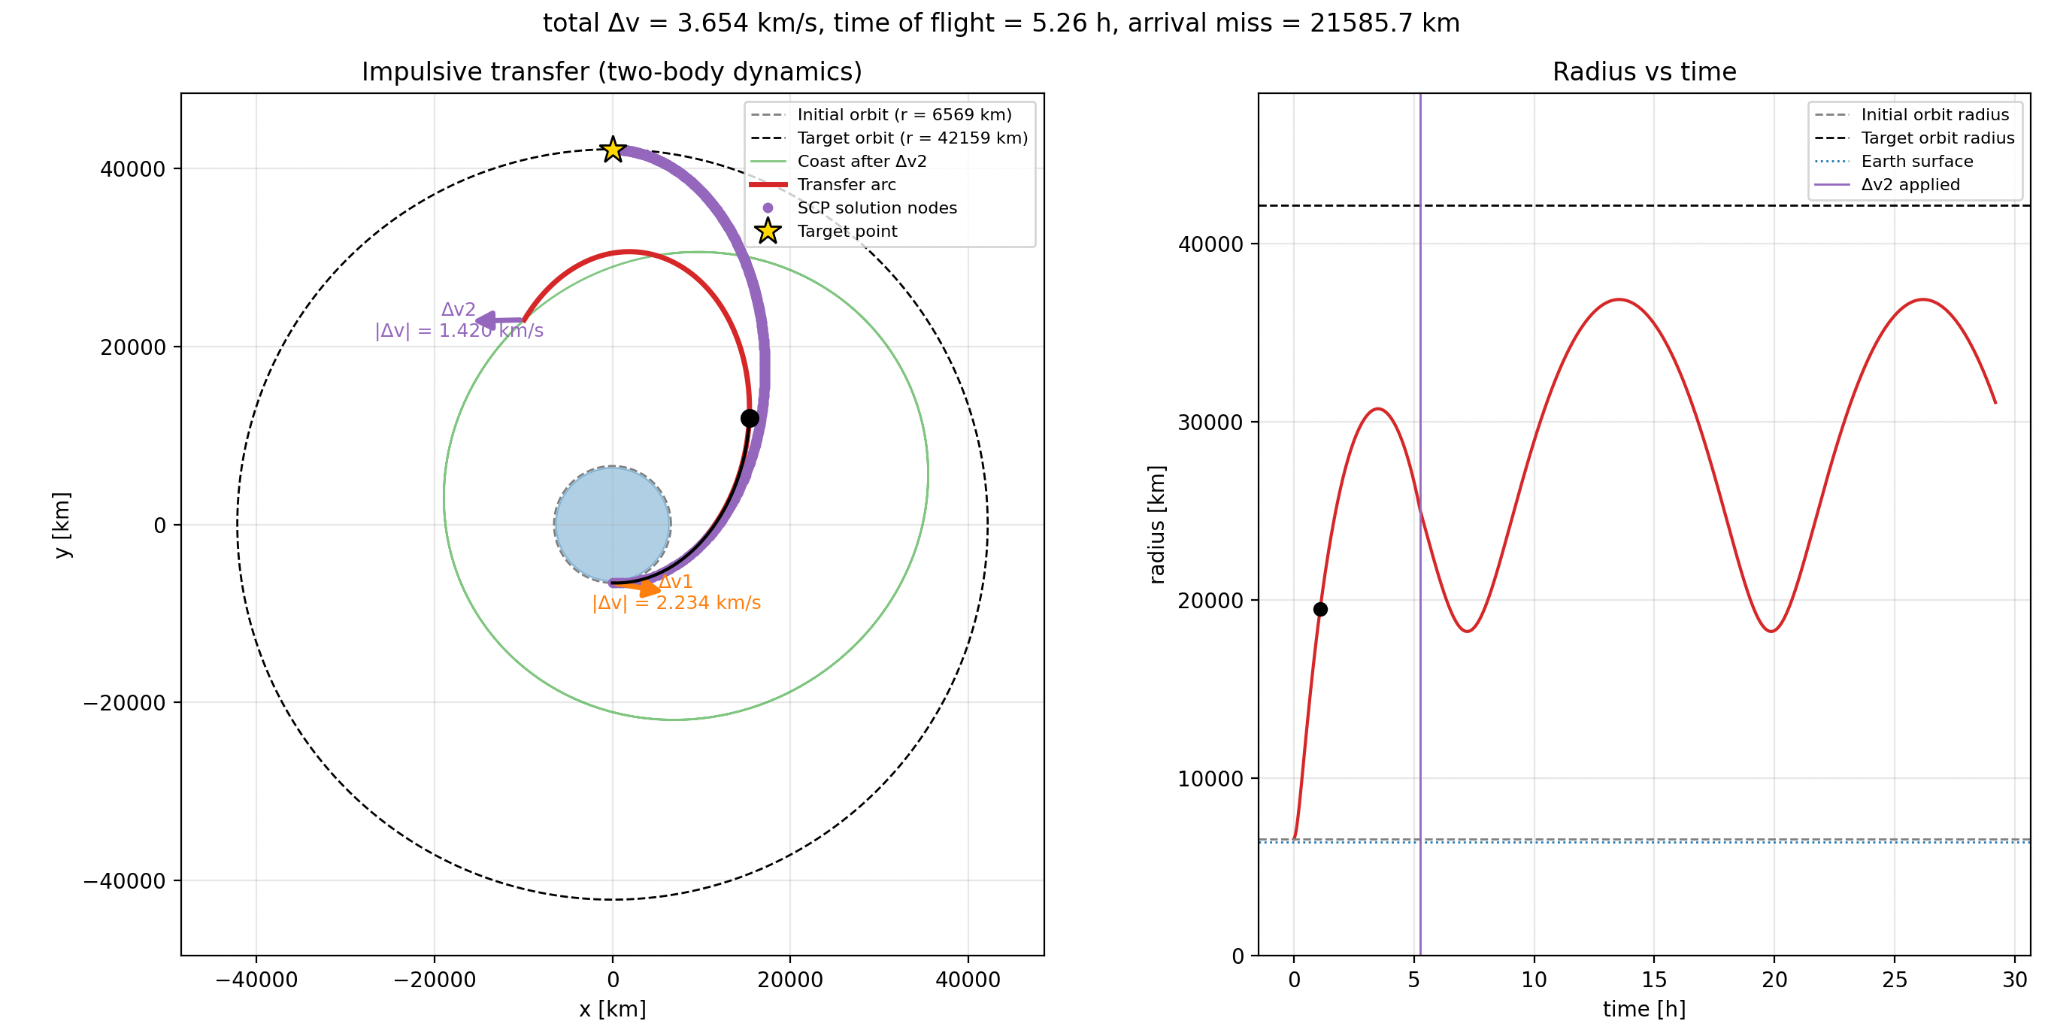
\includegraphics[width=0.85\textwidth]{figures/forward_euler_updated.png}
\caption{Forward Euler: $\Delta v=3.654$ km/s, $t_H=5.26$ h, and a propagated arrival miss of $21585.7$ km. The red nonlinear trajectory differs from the purple SCP nodes.}
\label{fig:euler}
\end{figure}

\subsection{Trapezoidal Integration}

Figure~\ref{fig:trap} shows the result with trapezoidal integration. The total burn is now $3.932$ km/s, compared with $3.935$ km/s analytically. The arrival miss is also much smaller at $205.7$ km. The propagated trajectory is close to the desired transfer orbit, although the $205.7$ km miss shows that the solution still needs work.

\begin{figure}[H]
\centering
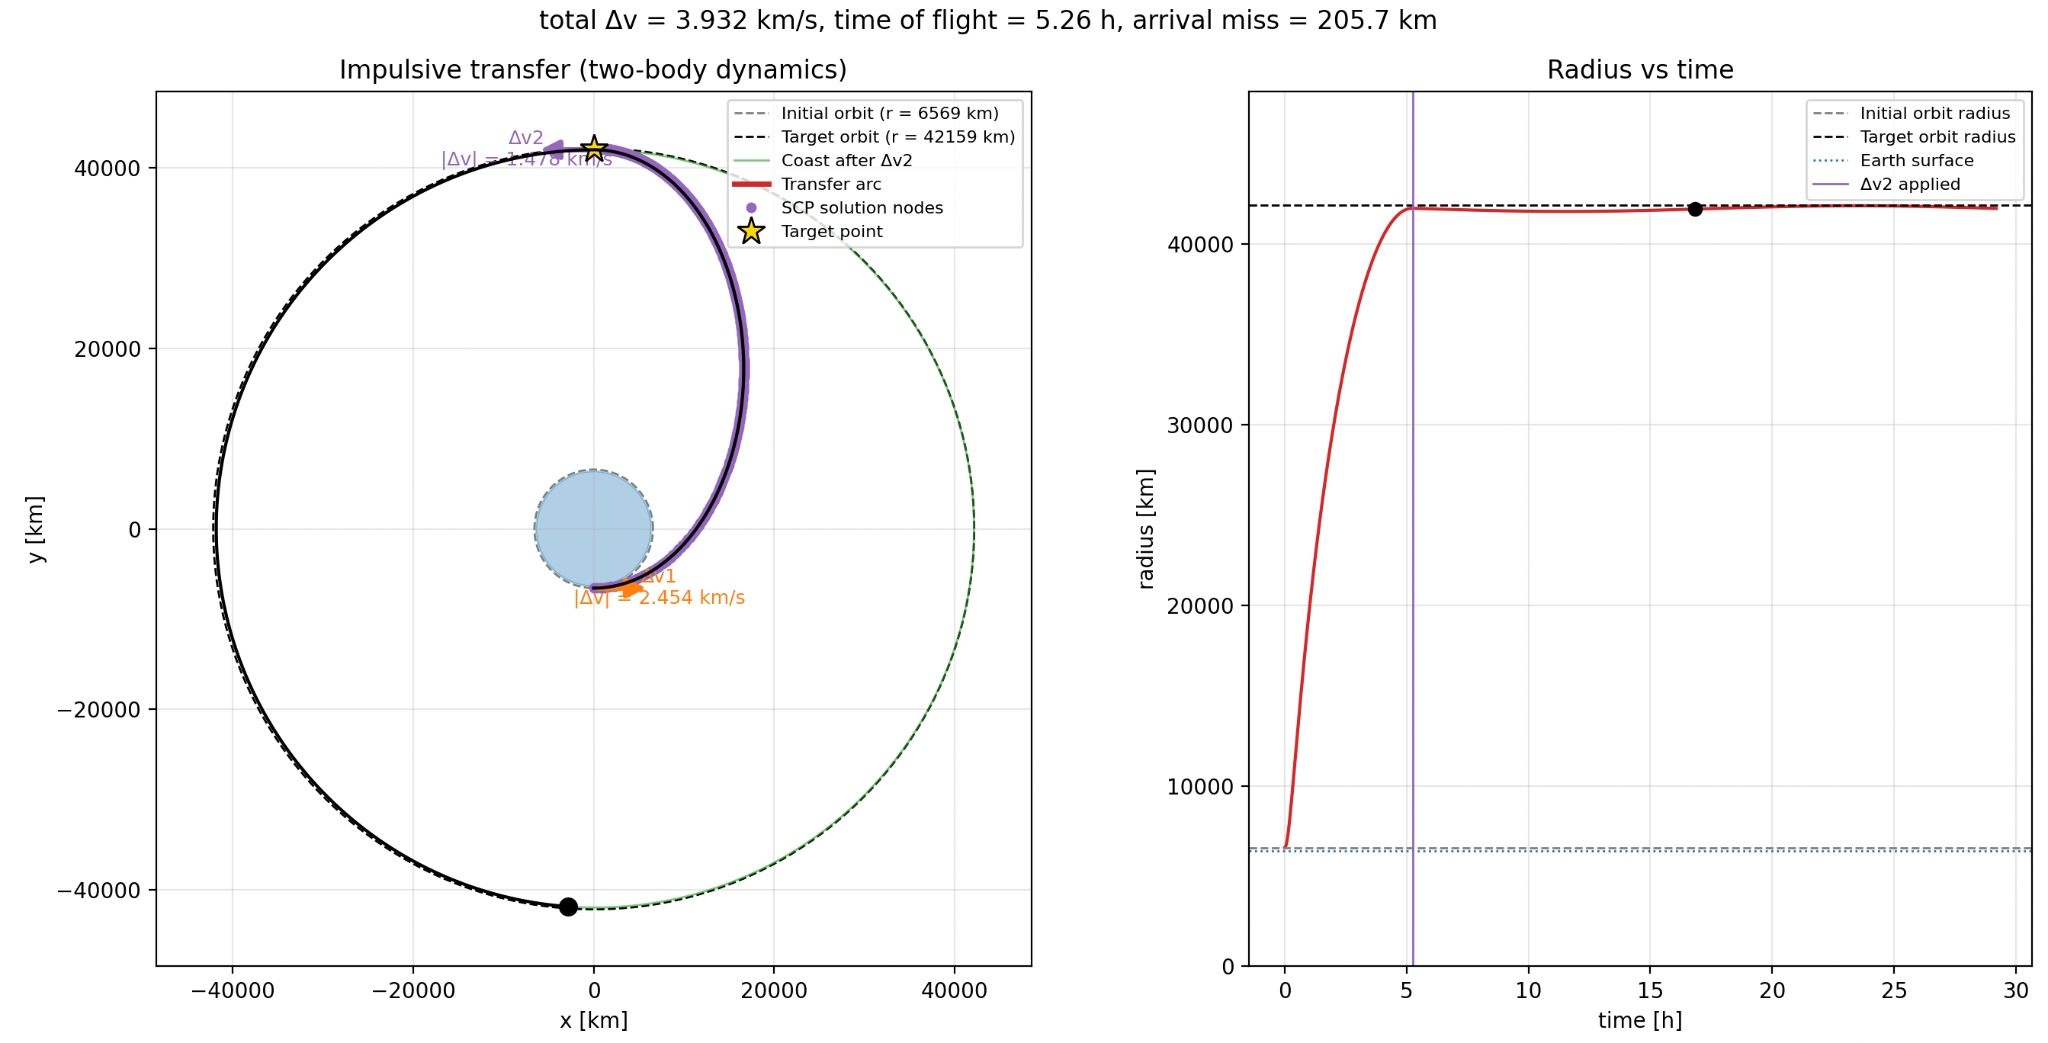
\includegraphics[width=0.85\textwidth]{figures/trapezoidal_updated.png}
\caption{Trapezoidal integration: $\Delta v=3.932$ km/s, $t_H=5.26$ h, and a propagated arrival miss of $205.7$ km. The nonlinear trajectory is much closer to the target orbit.}
\label{fig:trap}
\end{figure}

\end{document}
